\documentclass[12pt,a4paper]{scrartcl}
\usepackage[latin1]{inputenc}
\usepackage{amsmath}
\usepackage{amsfonts}
\usepackage{amssymb}
\usepackage{cancel}
\usepackage[english]{babel}
\usepackage{graphicx}
\usepackage{geometry}
\usepackage{afterpage}
\usepackage{rotating}
\usepackage{tabularx}
\usepackage{ltablex}
\usepackage{tikz}
\usepackage{float}
\usepackage{wrapfig}
\usepackage{booktabs}
\usepackage{array}
\usepackage{hyperref}
\usepackage{multirow}
\usepackage{parskip}
\usepackage{bbm}
\usepackage{pdflscape}
\usepackage{placeins}
\usepackage{flafter}
\usepackage{listings}
\usepackage[margin=10pt, font=scriptsize, labelfont=bf, labelsep=endash, position=bottom, format=hang, justification=raggedright,skip=3pt]{caption}
\let\stdsection\section
% \renewcommand\section{\newpage\stdsection}
\usepackage{subcaption}
\usepackage[comma]{natbib}
\bibpunct{(}{)}{;}{a}{}{,}
\bibliographystyle{/Users/matu/Documents/Literature/evolution}
%\DeclareMathOperator{\erfc}{erfc}

\usepackage[T1]{fontenc}

\newcommand{\mockalph}[1]{}
%\makeatletter
%\def\fixedlabel#1#2{%
%  \@bsphack%
%  \protected@write\@auxout{}%
%         {\string\newlabel{#1}{{#2}{\thepage}}}%
%  \@esphack}
%\makeatother

\makeatletter
\def\fixedlabel#1#2{%
  \@bsphack
  \begingroup
    \@onelevel@sanitize\@currentlabelname
    \edef\@currentlabelname{%
      \expandafter\strip@period\@currentlabelname\relax.\relax\@@@%
    }%
    \phantomsection%
    \protected@write\@auxout{}{%
      \string\newlabel{#1}{%
        {#2}%
        {\thepage}%
        {#2}%
        {\@currentHref}{}%
      }%
    }%
  \endgroup
  \@esphack
}
\makeatother

\newcommand{\codelst}{\begingroup
  \catcode`_=12 \docodelst}
\newcommand{\docodelst}[1]{%
  \lstinputlisting[caption=\texttt{#1}]{#1}%
  \endgroup
}

\newcommand{\specialcell}[2][c]{%
  \begin{tabular}[#1]{@{}c@{}}#2\end{tabular}}

\newcommand{\mc}[3]{\multicolumn{#1}{#2}{#3}}

%Line numbering and double-spaced lines
%
%\usepackage[pagewise]{lineno}
%\usepackage{lineno}
%%%%\modulolinenumbers[2]
%%%
%\linenumbers
%\let\stdsection\section
%%
%\usepackage{setspace}
%%%%%\onehalfspacing
%\doublespacing


\graphicspath{ {Figures/} }

\begin{document}
% \parindent 0mm
% \parskip 0mm
 \titlehead{empiricIST: An Integrated Software and analysis Tool for analyzing time-sampled sequence data such as EMPIRIC}
  \subject{README}
  \title{empiricIST: An Integrated Software and analysis Tool for analyzing time-sampled sequence data such as EMPIRIC}
  \author{Sebastian Matuszewski, Jeffrey D. Jensen and Claudia Bank}
  \date{Lausanne, \today}
\begingroup
 \makeatletter
 \@titlepagetrue
 \maketitle
\endgroup
\newpage
\tableofcontents
\newpage

\section{Introduction}


This program serves as an extension of the Bayesian Monte Carlo Markov chain (MCMC) method described in \cite{BanHW14} for estimating selection coefficients (growth rates) from engineered-mutation-driven experimental evolution data. These data are based on methods -- such as EMPIRIC -- in which specific mutations are introduced and compared against each other and the wildtype. All mutants (and the wildtype) are assumed to have evolved together in bulk culture for a number of generations with samples taken throughout the course of the experiment. Growth rates -- and thus the selection coefficient of each mutation -- can then be estimated from the number of reads obtained from deep sequencing.
The motivation for the \emph{empiricIST} software package is to provide an integrative framework for the analysis of experimental evolution data, and includes separate programs for processing raw sequence data and correcting for sequencing errors, obtaining statistically meaningful estimates of selection coefficients in a fast and efficient manner, and for providing ready-to-use summary statistics of the MCMC analysis and its associated parameter estimates.
It is highly advisable to read the two accompanying papers by \cite{BanHW14} and \cite{MatJB15} that describe the methods and underlying assumptions in more detail before using the software.

\section{Input data}

The \texttt{empiricIST\char`_MCMC} program only takes files in csv-format (comma-separated values) as input, which, furthermore, need to match a specified format (e.g., line endings need to be UNIX specific; input data needs to be ordered in a specified way). However, as part of the \emph{empiricIST} software package, we provide a python script -- \texttt{empiricIST\char`_MCMC\char`_Input.py} -- that adjusts the raw data to match the specific input format needed for the MCMC simulation program (including other options discussed in more detail below). A minimal example of the raw data that is required to generate the \texttt{empiricIST\char`_MCMC} input file is depicted in Figure~\ref{fig:RawInput}. Note that the raw data itself also needs to be csv-formatted with column entries separated by a comma (','), a semi-colon (';') or a tab ('\\t').
Furthermore, the raw data file needs to have (exactly) one column either called 'sequence', 'Sequence', 'seq' or 'Seq' with at least two rows (the wild-type reference and a mutant) and at least additional 3 columns (i.e., time points) corresponding to the number of sequencing reads, with respectively named header cells.

\begin{figure}
\centering 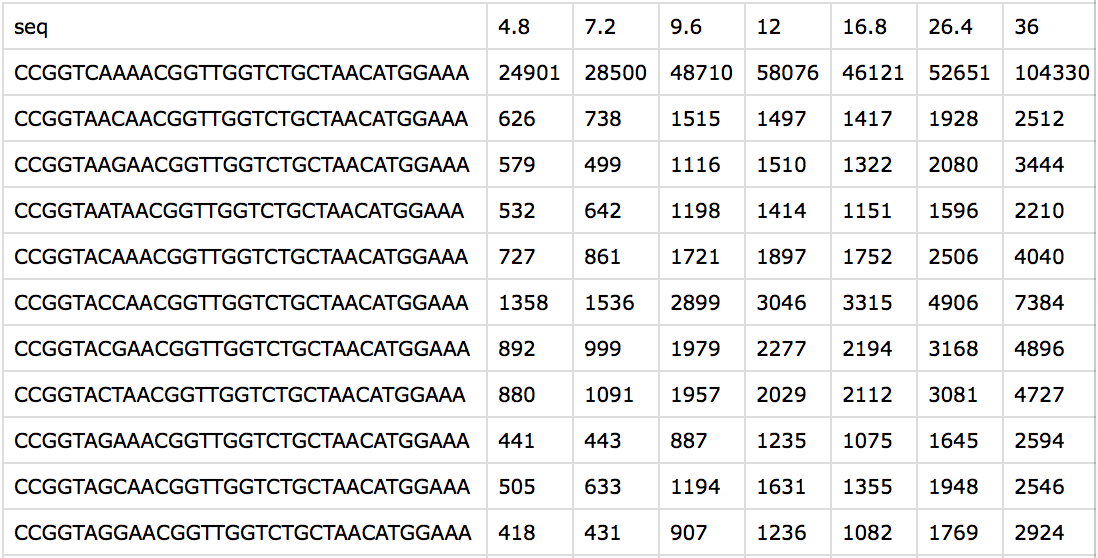
\includegraphics[width=0.65\textwidth]{RawDataInput.png}
\caption{Schematic illustration of the minimal data needed to run the \texttt{empiricIST\char`_MCMC} program. \label{fig:RawInput}}
\end{figure}

\subsection{\texttt{empiricIST\char`_MCMC\char`_Input}.py}

The program \texttt{empiricIST\char`_MCMC\char`_Input.py} is written in Python (2.7) and serves as a link between the (raw) time-sampled sequence data (e.g., obtained from EMPIRIC) and the \texttt{empiricIST\char`_MCMC} simulation program for the estimation of mutant growth rates 'r'. While it primarily ensures that the input data matches the input format required by the MCMC simulation program, it comes with additional options that will be detailed here.

The general usage is as follows: After opening a command-line interface (e.g., Shell, Terminal) and navigating to the location of the \texttt{empiricIST\char`_MCMC\char`_Input.py} file, the program can be executed by typing
\begin{lstlisting}
python empiricIST_MCMC_Input.py [options] .
\end{lstlisting}

Note that this requires that the 'PATHVARIABLE' for Python has been set correctly on your system. Please consult the online Python documentation for further details (https://docs.python.org/2/). Without specifying any options the program will exit with an error and provide a short documentation on its usage, as it requires the name of a (raw) data input file and the start of the sequencing read data table to be specified (by invoking the '-f' and '-s' option, respectively). All options and their usage are given in Table~\ref{tbl:tablePythonOptions}.

{
\centering
\renewcommand{\arraystretch}{1.25}
\begin{scriptsize}
\begin{tabularx}{1\textwidth}{>{\raggedright\arraybackslash}m{1.6cm} >{\raggedright\arraybackslash}m{2.5cm} >{\raggedright\arraybackslash}m{8.2cm}}
\caption{A summary of the options of the \texttt{empiricIST\char`_MCMC\char`_Input.py} program.}
\label{tbl:tablePythonOptions}\\
\toprule
\mc{1}{l}{\textbf{Short/Long option}} & \textbf{Accepted values} & \textbf{Description} \\
 & & \\\hline
\mc{1}{l}{-h, --help} & none & 
\hangindent=1em
\hangafter=1
\noindent
When the '-h'-option is invoked, a short documentation on the usage of the program is shown. Note that, if this option is invoked, the python program is not executed.
\\
\mc{1}{l}{-f, --file=} & string  &
\hangindent=1em
\hangafter=1
\noindent
The '-f'-option is a mandatory option, which passes the name of the (raw) data input file (csv formatted) to the python program. Files created by the python program will take the name of the input file and add option-dependent specific file identifiers. 
\\
\mc{1}{l}{-s, --skipcol=} & integer &
\hangindent=1em
\hangafter=1
\noindent
The '-s'-option is a mandatory option, which takes an integer value corresponding to the number of descriptive columns that precede the actual 'data matrix' of sequencing read counts. For example, for the raw data depicted in Figure~\ref{fig:RawInput}, the user would have to pass '-s 1' (or equivalently '--skipcol=1'). Please note that the data matrix must always span all remaining columns.
\\
\mc{1}{l}{-o, --outlier=} & 'detect' or 'impute' &
\hangindent=1em
\hangafter=1
\noindent
When the '-o'-option is invoked, the python program will perform an outlier analysis. If '-o detect' (or equivalently '--outlier=detect'), the python program performs a log-linear regression analysis for all mutants. Data points are then classified as outliers on the basis of the DFBeta statistic with a cut-off value of 2 (with data points surpassing this cut-off regarded as outliers). For more details please consult \cite{BanHW14}.
If '-o impute' (or equivalently '--outlier=impute'), the python program performs a log-linear regression analysis for all mutants. Data points are then classified as outliers on the basis of the DFBeta statistic with a cut-off value of 2 and their studentized residuals with a cut-off value of 3 (with data points surpassing \emph{both} cut-offs are regarded as outliers) and imputed as described in \cite{MatJB15}. Furthermore, an additional output file -- whose name consists of 'ImputedData' along with the input file name -- is produced that lists all imputed data points. In particular, the output is a simple matrix where rows denote different mutants and columns correspond to the different time points. An entry of  '1' indicates that the data has \emph{not} been imputed; an entry of '0' indicates that the data point has been imputed.
\\
\mc{1}{l}{-l, --leadseq=} & integer &
\hangindent=1em
\hangafter=1
\noindent 
When the '-l'-option is invoked, the first 'integer' characters, that precede the original mutant sequence (e.g., sites that function as DNA barcode or sequence tag), are removed.
\\
\mc{1}{l}{-t, --trailseq=} & integer &
\hangindent=1em
\hangafter=1
\noindent 
When the '-l'-option is invoked, the first 'integer' characters, that trail the original mutant sequence (e.g., sites that function as DNA barcode or sequence tag), are removed.
\\
\mc{1}{l}{-p, --pool} & none &
\hangindent=1em
\hangafter=1
\noindent
When the '-p'-option is invoked, the DNA-sequences (characterizing the different mutants) are translated into amino acids. The data is then pooled based on their amino acid sequence, assuming that identical amino acid sequences, though differing in their DNA sequence (synonymous mutants), have the same growth rate (but different initial population sizes). Note that even if the '-p'-option is not invoked, data is pooled based on the sequence name (which can be any string and not only letters from the DNA alphabet). 
\\ 
\mc{1}{l}{-e, --exp} & none &
\hangindent=1em
\hangafter=1
\noindent
When the '-e'-option is invoked, time points are taken to be in hours instead of generations (i.e., the default).
\\
\mc{1}{l}{-g, --group=} & integer &
\hangindent=1em
\hangafter=1
\noindent
When the '-g'-option is invoked, the data is grouped into subsets of mutants each of minimal size 'integer'. This results in more data sets with less mutants, such that the per-data set computation time is reduced, without affecting parameter estimates or the shape of the log-likelihood surface (compared to analysis of the full data set). The program also ensures, that mutants with identical mutant or protein ID (i.e., mutants that have an identical DNA- or amino acid sequence) remain in the same data sub-set as they are assumed to evolve under an identical growth rate (r). In general, the last line of the resulting input file serves as a summary line (indicated by a '-1' as mutant/protein ID and by 'XXX' in the sequence column) that gives the number of all sequencing reads not in the current sub-set (but which are still needed to be accounted for). 
Estimates for the growth rates and the selection coefficients for the summary line are not calculated (but simply equated to those of the reference strain), since MCMC simulation estimates for this 'summary mutant' will later be discarded. The name of the output file (i.e., the MCMC input file) is composed of the standard output file identifier 'MCMCInput', the grouping identifier (a consecutive number of the sub data sets created) and the name of the input file. 
\\
\mc{1}{l}{-i, --initialize} & none &
\hangindent=1em
\hangafter=1
\noindent
When the '-i'-option is invoked, and additional input file is created that specifies the initial growth rates (r) and initial population sizes (c) for all mutants based on he log-linear regression. Note that this could potentially bias the MCMC algorithm, since the initial starting point of the Markov chain could be trapped in a local log-likelihood optimum. Often, however, the median of the growth rates and the initial population sizes from the MCMC-DFE simulations are close enough to the corresponding estimates from the log-linear regression such that starting at these values could shorten the burn-in period and, thus, reduce the run time. For mutants with identical DNA or amino acid sequence, the mean initial population size is calculated (from these mutants) and taken as the starting value for the MCMC simulation program. Given the estimated mean initial population size, the growth rate is estimated from the log-linear regression.
The name of the output file is composed of the standard output file identifier 'MCMCInput', an optional grouping identifier (see '-g'-option), the name of the input file, and an initialization file identifier '\texttt{\char`_inputRC}'. 
\\
\end{tabularx}
\end{scriptsize}
}

An illustration of the output file produced by the python program (i.e., the input file for the MCMC simulation program) is depicted in Figure~\ref{fig:PythonOutput}.

\begin{figure}
\centering 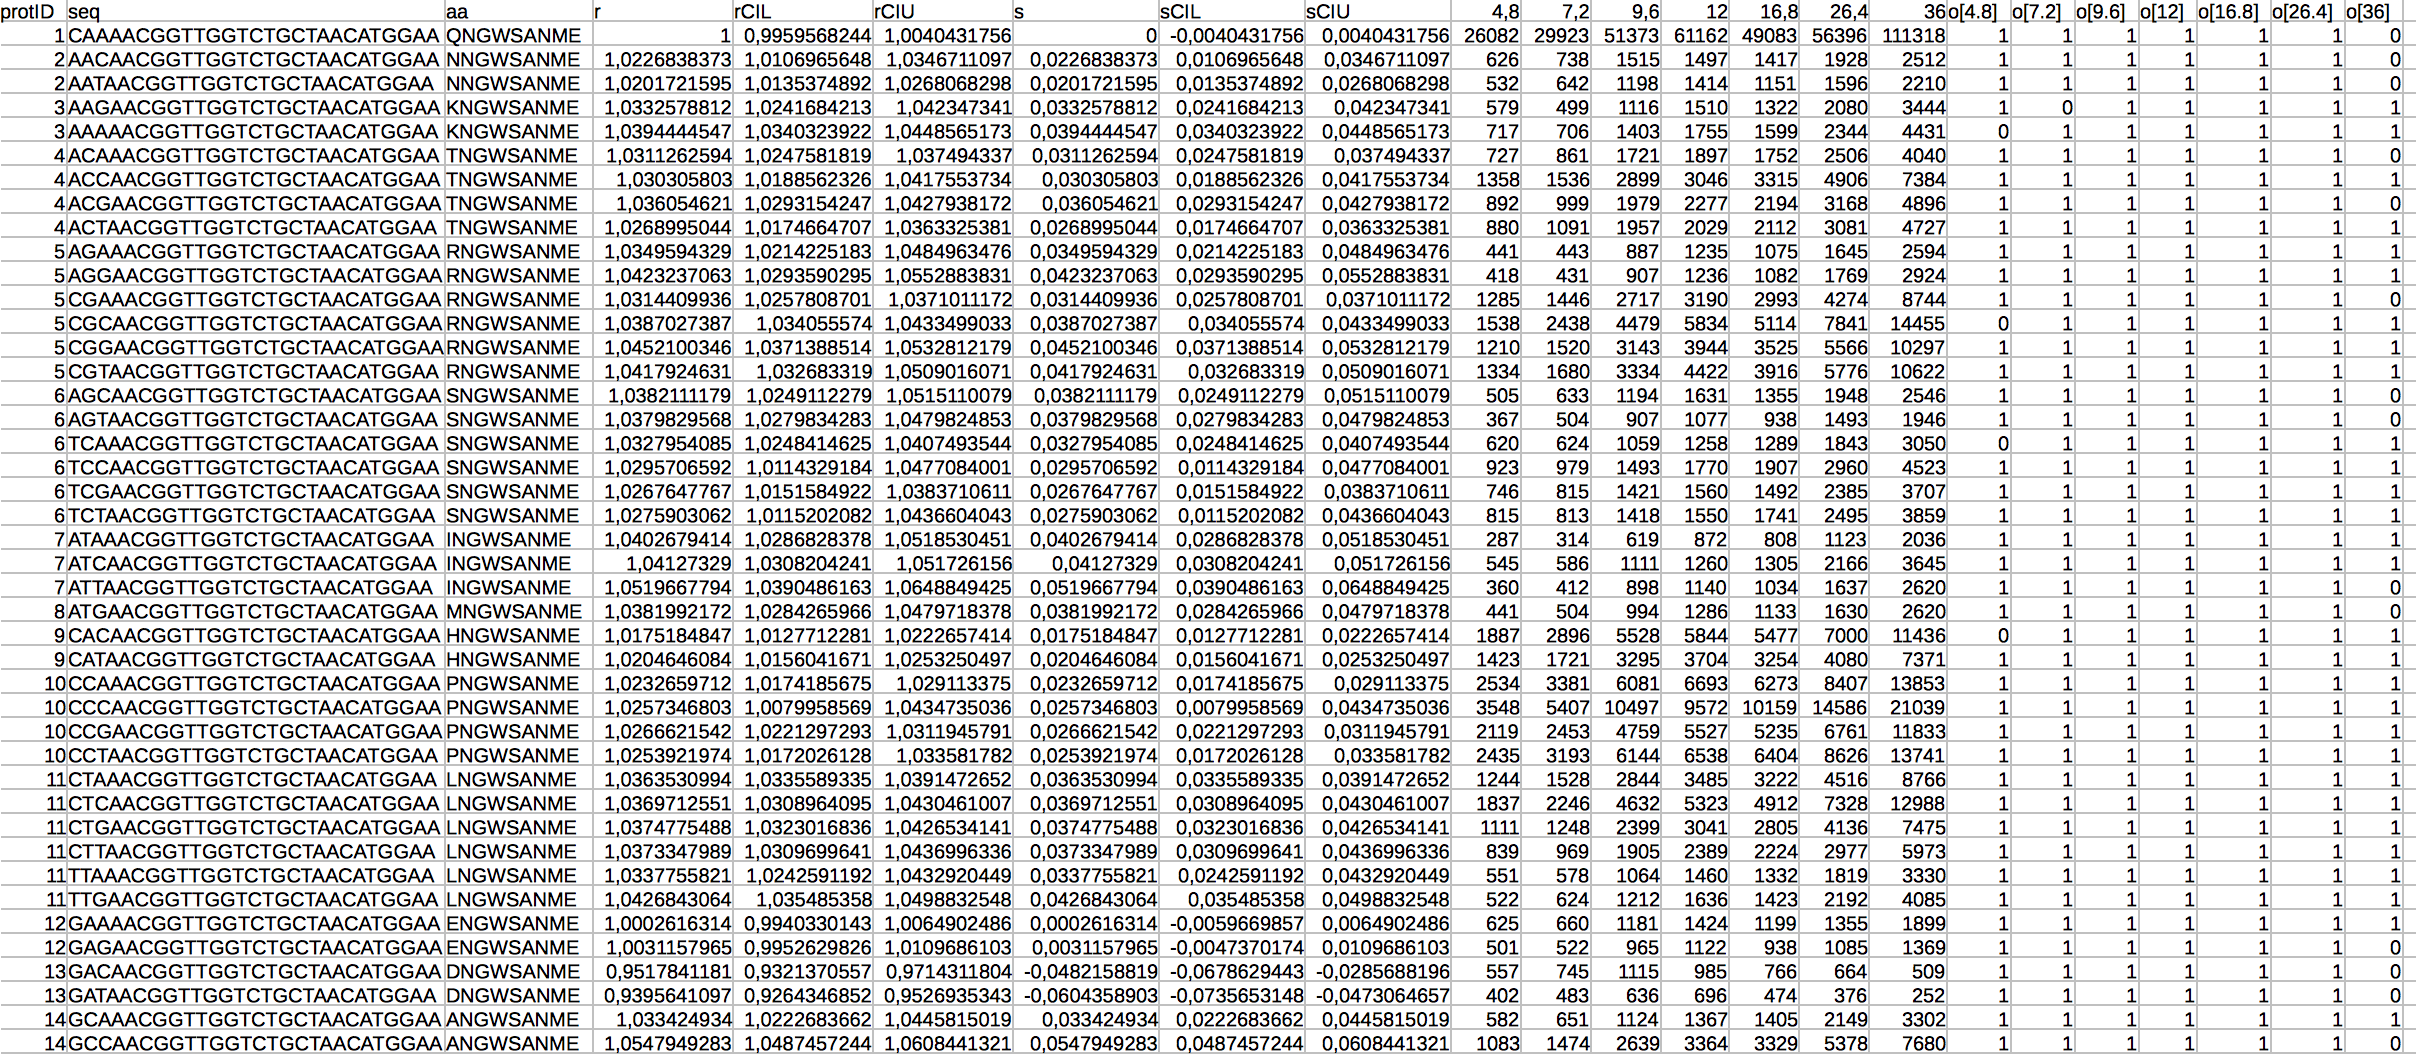
\includegraphics[width=0.95\textwidth]{MCMC-InputExample.png}
\caption{Schematic illustration of the output produced by the python program and which serves as input for the MCMC simulation program. This input data has been created using the minimal raw data shown in Fig.~\ref{fig:RawInput}, where the first five bases and the last base have been discarded (barcodes; '-l' and '-t' option). DNA sequences ('seq' column) have been translated to amino acids ('aa' column) and pooled ('-p' option), such that identical amino acid sequences have the same protein ID ('protID' column). Estimates of the growth rates 'r' ('r' column) and the selection coefficient 's' ('s' column) along with the $95\%$-confidence intervals are based on the log-linear regression (where 'rCIL' and 'rCIU' give the lower and upper boundary of the confidence interval for the growth rate r, respectively. Notation is analogous for the selection coefficient 's'.). Please note, that while the MCMC simulation program assumes that mutants with identical sequence information (i.e., for sequences with identical 'protID') evolve at the same growth rate, log-linear estimates for 'r' and 's' are based on individual mutants.
The columns '4.8', '7.2', '9.6', '12', '16.8', and '26.4' give the number of sequencing reads obtained from sampling at these time points for each mutant (row). If the '-o detect'-option is invoked, the matrix of sequencing reads is followed by an outlier matrix for the corresponding time points and mutants, where '0' indicate data points that where classified as outliers.\label{fig:PythonOutput}}
\end{figure}

Depending on the invoked options, the name of the MCMC simulation input file that is produced by the python program is given by the standard output file identifier 'MCMCInput', an optional grouping identifier (see '-g'-option) and the name of the raw data file.

\section{Usage} 
 
We provide executables for (Mac OS X), Windows and Linux. The C++ source code along with a system specific makefile are provided under a GNU General Public License as published by the Free Software Foundation. If you do not need to compile the program yourself you can skip the next subsection.
 
\subsection{Compilation} 

Note that compilation requires that the (Gnu Scientific Library) (gsl-library) is installed on your system. Information on how to install the gsl-library can be found under \url{http://www.gnu.org/software/gsl/}.
On Windows the easiest way to obtain the gsl-library is to install Cygwin (\url{http://www.cygwin.com/}) including the developers (all) packages. Alternatively, MinGW (\url{http://www.mingw.org/}) provides a ''minimalist GNU for Windows'' development environment. Under MinGW though, the gsl-library needs to be installed independently. A short instruction is given in the following paragraph.

Compilation of the program has successfully been tested on MacOSX (10.9.5) using 'clang' (version 6.0) and 'gcc' (version 4.9), on Ubuntu (14.04 LTS) using 'g++' (version 4.8.2), and on Windows (8.1) using 'g++' (version 4.8.1 under MinGW; version 4.9.2 under Cygwin).

\subsubsection*{Windows}

\paragraph*{Cygwin}
Please note that Cygwin is a large collection of GNU and open source tools, which provide functionality similar to a Linux distribution on Windows. Thus, when using Cygwin, commands and folder navigation are different to those from a native Windows Shell (e.g., Powershell).
For example, under Cygwin you first need to type 
\begin{lstlisting}
cd /cygdrive/c
\end{lstlisting}
to navigate to the drive 'C:\textbackslash'.

The easiest way to compile the program is by using the provided makefile. After navigating to the folder where the source code is stored, simply type
\begin{lstlisting}
make -f Makefile_MCMC_Cygwin .
\end{lstlisting}
Please note that you might want to adjust the makefile, in particular, to change the name of the executable which is by default set to '\texttt{empiricIST\char`_MCMC\char`_Cygwin.exe}'.

Alternatively, you can manually compile the program from source by navigating to the folder where the source code is stored and by typing
\begin{lstlisting}
g++ empiricIST_MCMC.cpp -lgsl -lgslcblas -O3 -o 'NameOfProgram' ,
\end{lstlisting}
where 'NameOfProgram' should be replaced by the actual name of the compiled program (e.g., \texttt{empiricIST\char`_MCMC}). 

Note that Cygwin does not allow to link libraries statically.

\paragraph*{MinGW}
Please note that MinGW provides a complete open source programming tool set for the development of native Windows applications (including both different compilers and a ``minimal system'' bourne shell command line interpreter system MSYS).

\subparagraph{Compilation and installation of the gsl-library from source}
Before compilation and installation of the gsl-library please read and follow the installation instructions provided with the most recent version of gsl.

\begin{enumerate}
\item Download the latest version of gsl from \url{http://ftpmirror.gnu.org/gsl/}
\item Navigate to the place where the downloaded tar archive is stored and unpack it by typing 
\begin{lstlisting}
tar -zxvf gsl-x.xx.tar.gz ,
\end{lstlisting}
where 'x.xx' should be replaced by the version number.
\item Navigate to 'gsl-x.xx/' and carefully read the 'INSTALL' document and follow the instructions to configure, make and install the gsl-library:
\begin{lstlisting}
./configure
make
make install
\end{lstlisting}
\item GSL binaries, headers and library files are installed automatically in the 'bin/', 'include/gsl/', and 'lib/' subdirectories (if not specified otherwise; in that case you would also need to adjust the linker and compiler flags in the makefile).
\end{enumerate}

\subparagraph{Compilation of the MCMC}

Open a MSYS shell and type
\begin{lstlisting}
cd /c
\end{lstlisting}
to navigate to the drive 'C:\textbackslash'.

The easiest way to compile the program is by using the provided makefile. After navigating to the folder where the source code is stored simply type
\begin{lstlisting}
make -f Makefile_empiricIST_MCMC_WINDOWS .
\end{lstlisting}
Please note that you might want to adjust the makefile, in particular, to change the name of the executable which is by default set to '\texttt{empiricIST\char`_MCMC.exe}'.

Alternatively, you can manually compile the program from source by navigating to the folder where the source code is stored and by typing
\begin{lstlisting}
g++ empiricIST_MCMC.cpp -lgsl -lgslcblas -O3 -o 'NameOfProgram' ,
\end{lstlisting}
where 'NameOfProgram' should be replaced by the actual name of the compiled program (e.g., \texttt{empiricIST\char`_MCMC}). 


\subsubsection*{Linux}

The easiest way to compile the program is by using the provided makefile.
Use the Shell to navigate to the folder where the source code is stored and simply type 
\begin{lstlisting}
make -f empiricIST_MCMC_Linux .
\end{lstlisting}
Please note that you might want to adjust the makefile, in particular, to change the name of the executable which is by default set to '\texttt{\emph{empiricIST}\char`_MCMC}'.

Alternatively, you can manually compile the program from source by navigating to the folder where the source code is stored and by typing
\begin{lstlisting}
g++ empiricIST_MCMC.cpp -lgsl -lgslcblas -O3 -o 'NameOfProgram' ,
\end{lstlisting}
where 'NameOfProgram' should be replaced by the actual name of the compiled program (e.g., \texttt{empiricIST\char`_MCMC}). 

\subsubsection*{Mac OS X}

The easiest way to compile the program is by using the provided makefile.
Use the Terminal to navigate to the folder where the source code is stored and simply type 
\begin{lstlisting}
make -f empiricIST_MCMC_MacOSX .
\end{lstlisting}
Please note that you might want to adjust the makefile, in particular, to change the name of the executable which is by default set to '\texttt{empiricIST\char`_MCMC}'.

Alternatively, you can manually compile the program from source by navigating to the folder where the source code is stored and by typing
\begin{lstlisting}
g++ empiricIST_MCMC.cpp -lgsl -lgslcblas -O3 -o 'NameOfProgram' ,
\end{lstlisting}
where 'NameOfProgram' should be replaced by the actual name of the compiled program (e.g., \texttt{empiricIST\char`_MCMC}). 
 
\subsection{Execution}
 
Note that the \texttt{\emph{empiricIST}\char`_MCMC} program is a command line program which is run from a command-line interface (e.g., Shell, Terminal, Powershell), with arguments and parameters being passed over the command line. An overview and description of the parameters can be found in Table~\ref{tbl:tableParameterDescription}.
Depending on your operating system there are different ways to call the program. These will be explained in the subsequent paragraphs.
 
\subsubsection*{Windows}
 
\paragraph{Cygwin}

There are two ways to execute the program. First, the easiest way is to use the provided bash script '\texttt{empiricIST\char`_MCMC\char`_Cygwin.sh}', where the parameters (e.g., 'PathToDataFile', skipCol, burnin) can be specified by the user.
To begin, navigate to the folder where the executable and the bash script are stored and type
\begin{lstlisting}
./empiricIST_MCMC_Cygwin.sh .
\end{lstlisting}

Second, you can manually execute the program by using Cygwin to navigate to the folder where the executable is stored and typing
 \begin{lstlisting}[breaklines=true] 
./'NameOfProgram' 'PathToDatafile' outfileName skipCol outliersPresent burnin subsampling noSets set proposalDistCScale proposalDistRSD initialRC printLogLTS printESS printOutput timeHours seed ,
\end{lstlisting}  
where the parameters (e.g., 'PathToDataFile', skipCol, burnin) need to be specified by the user. 

Note that under Cygwin the 'PathToDataFile' needs to be preceded by '/cygdrive/c/' (if the datafile is stored on the 'c' drive).

\paragraph{Powershell}

There are two ways to execute the program. First, the easiest way is to use the provided powershell script '\texttt{empiricIST\char`_MCMC\char`_WINDOWS.ps1}', where the parameters (e.g., 'PathToDataFile', skipCol, burnin) can be specified by the user.
To begin, open Powershell and navigate to the folder where the executable and the powershell script are stored and type
\begin{lstlisting}
& empiricIST_MCMC_WINDOWS.ps1 .
\end{lstlisting}

Second, you can manually execute the program by using Powershell to navigate to the folder where the executable is stored and typing
 \begin{lstlisting}[breaklines=true] 
& 'NameOfProgram' 'PathToDatafile' outfileName skipCol outliersPresent burnin subsampling noSets set proposalDistCScale proposalDistRSD initialRC printLogLTS printESS printOutput timeHours seed ,
\end{lstlisting}  
where the parameters (e.g., 'PathToDataFile', skipCol, burnin) need to be specified by the user. 

\subsubsection*{Linux}

There are two ways to execute the program. First, the easiest way is to use the provided bash script '\texttt{\emph{empiricIST}\char`_MCMC\char`_Linux.sh}', where the parameters (e.g., 'PathToDataFile', skipCol, burnin) can be specified by the user.
To begin, navigate to the folder where the executable and the bash script are store and type
\begin{lstlisting}
./empiricIST_MCMC_Linux.sh .
\end{lstlisting}

Second, you can manually execute the program by using the shell to navigate to the folder where the executable is stored and typing
 \begin{lstlisting}[breaklines=true] 
./'NameOfProgram' 'PathToDatafile' outfileName skipCol outliersPresent burnin subsampling noSets set proposalDistCScale proposalDistRSD initialRC printLogLTS printESS printOutput timeHours seed ,
\end{lstlisting}  
where the parameters (e.g., 'PathToDataFile', skipCol, burnin) need to be specified by the user. 

\subsubsection*{Mac OS X}
 
There are two ways to execute the program.  First, the easiest way is to use the provided bash script  '\texttt{\emph{empiricIST}\char`_MCMC\char`_MacOSX.sh}', where the parameters (e.g., 'PathToDataFile', skipCol, burnin) can be specified by the user.
To begin, navigate to the folder where the executable and the bash script are store and type
\begin{lstlisting}
./empiricIST_MCMC_MacOSX.sh .
\end{lstlisting} 

Second, you can manually execute the program by using the terminal to navigate to the folder where the executable is stored and typing 
 \begin{lstlisting}[breaklines=true] 
./'NameOfProgram' 'PathToDatafile' outfileName skipCol outliersPresent burnin subsampling noSets set proposalDistCScale proposalDistRSD initialRC printLogLTS printESS printOutput timeHours seed ,
\end{lstlisting}  
where the parameters (e.g., 'PathToDataFile', skipCol, burnin) need to be specified by the user. 

 
{
\centering
\begin{scriptsize}
\renewcommand{\arraystretch}{1.25}
\begin{tabularx}{1\textwidth}{>{\raggedright\arraybackslash}m{1.6cm}>{\raggedright\arraybackslash}m{2.6cm}>{\raggedright\arraybackslash}m{8.3cm}}
%\begin{tabularx}{\textwidth}{l l X}
\caption{A summary of the parameters of the MCMC program.}\label{tbl:tableParameterDescription}\\
\toprule
\mc{1}{l}{\textbf{Category}} & \textbf{Accepted values} & \textbf{Description} \\
\mc{1}{r}{\textbf{Parameter}} & & \\\hline
 &&\\
\mc{1}{l}{Data} &  & \\\cline{1-1}
\mc{1}{r}{datafile} & string &
\hangindent=1em
\hangafter=1
\noindent
Give the full path to the datafile \linebreak
(e.g., /users/me/PathToData/reads.csv).
\\
\mc{1}{r}{outfileName} & string &
\hangindent=1em
\hangafter=1
\noindent
Name of the output file. The program will take the name of the input file and add the 'outfileName', the time of execution and the identifier (e.g., '\texttt{\char`_C}').
This produces for example \linebreak
/PathToData/\texttt{\char`_'datafile'\char`_'outfileName'\char`_'date\&time'\char`_C.txt}. 
\\
\mc{1}{r}{skipCol} & integer, $\$\geq$0 &
\hangindent=1em
\hangafter=1
\noindent
Number of columns to skip in data file before read numbers start.
\\
\mc{1}{r}{outliersPresent} & bool &
\hangindent=1em
\hangafter=1
\noindent
If '0' there is no outlier matrix in the data file. If '1' there is an outlier matrix in the data file.
\\
\mc{1}{l}{MCMC} &  & \\\cline{1-1}
\mc{1}{r}{burnin} & integer, $\$\geq0$ & 
\hangindent=1em
\hangafter=1
\noindent
Number of accepted values that are discarded (burn-in period). During the burn-in period the parameters of the proposal distribution are adjusted.
\\
\mc{1}{r}{subSampling} & integer, $\$\geq0$ & 
\hangindent=1em
\hangafter=1
\noindent
After the burn-in period only every 'subSampling' accepted value is recorded (i.e., written to file).
\\
\mc{1}{r}{noSets} & integer, $\$\>0$ & 
\hangindent=1em
\hangafter=1
\noindent
Number of output data sets that are recorded each of size size 'setSize'. The total chain length is given by 'burnin'$+$'noSets'$\times$'setSize'$\times$'subSampling'.
\\
\mc{1}{r}{setSize} & integer, $\$\>0$ & 
\hangindent=1em
\hangafter=1
\noindent
Number of recorded samples per set. The total chain length is given by 'burnin'$+$'noSets'$\times$'setSize'$\times$'subSampling'. Output to file is written every 'setSize' accepted and recorded samples.
\\
%\mc{1}{r}{terminateESS} & integer & 
%\hangindent=1em
%\hangafter=1
%\noindent
%An alternative stopping condition. If '-1',  the total chain length is given by 'burnin'$+$'noSets'$\times$'setSize'$\times$'subSampling'. \linebreak
%If $\neq-1$, the MCMC stops when the minimal ESS for each sampled parameter has been reached. 
%\\
\mc{1}{r}{proposalDistCScale} & double, $\$>0$ & 
\hangindent=1em
\hangafter=1
\noindent
Scale parameter of the proposal distribution of initial population sizes 'c' (Cauchy distribution) .
\\
\mc{1}{r}{proposalDistRSD} & double, $\$>0$ & 
\hangindent=1em
\hangafter=1
\noindent
Standard deviation of the proposal distribution of growth rates 'r' (Normal distribution) .
\\
\mc{1}{r}{inititalRC} & string & 
\hangindent=1em
\hangafter=1
\noindent
An alternative way to initialize the growth rates 'r', the initial population sizes 'c' and to (optionally) set the parameters of the proposal distributions. This option allows, for example, to continue an MCMC run that has not been run long enough from the previous accepted sample. Note that for continuing an MCMC run the burn-in has to be set to 0. If 'initialRC' $= -1$, the default initialization is used (i.e., r=1 and initial population size = first observed read number for all mutants). When 'initialRC' $\neq -1$ the program will search for the initialization file
\texttt{'datafile'\char`_'initialRC'}. In particular if the 'datafile' has been specified as '/users/me/PathToData/reads.csv' and the name of the initialization file is '\texttt{\char`_reads\char`_initialRC.txt}', the initialRC parameter passed to the program should be 'initialRC.txt'. Note that this file needs to be located in the same directory as the datafile and that the name initialization file should be of the form \texttt{XYZData\char`_'initialRC'}.
\\
\mc{1}{r}{timeHours} & bool & 
\hangindent=1em
\hangafter=1
\noindent
If '0', time points are assumed to be measured in generation time. If '1', each time point is assumed to be measured  hours.
\\
\mc{1}{l}{Output} &  & \\\cline{1-1}
\mc{1}{r}{printLogLTS} & bool & 
\hangindent=1em
\hangafter=1
\noindent
If '0', no time series of log-likelihoods is written. If '1', a time series of log-likelihoods is written.
\\
\mc{1}{r}{printESS} & bool & 
\hangindent=1em
\hangafter=1
\noindent
If '0', no ESS statistics are written. If '1', ESS statistics are written. The effective sample size (ESS) is calculated every 1000 accepted samples.
\\
\mc{1}{r}{printOutput} & bool & 
\hangindent=1em
\hangafter=1
\noindent
If '0', no additional output will be written to screen. If '1', additional output will be written to screen. Mainly for inspection purposes.
\\
\mc{1}{l}{Random numbers} &  & \\\cline{1-1}
\mc{1}{r}{seed} & integer & 
\hangindent=1em
\hangafter=1
\noindent
Sets the random number seed. If 'seed'$\leq0$ a random number seed is created automatically based on computer run time.
\\
\end{tabularx}
\end{scriptsize}
}

\section{MCMC output}

The program creates different kinds of output files that contain time-series data for different parameters, summary and diagnostic statistics for those parameters and for the entire MCMC run.
Note that, even though all output files are plain 'txt'-files, they are all formatted as '.tsv'-files (tab separated) and can be displayed nicely with any spreadsheet application (e.g., Excel). Furthermore, all output files are structured such that they start with a list of the input/parameters for the MCMC run which are followed by the simulation results.

{
\clearpage
\centering
\begin{scriptsize}
\renewcommand{\arraystretch}{1.25}
\begin{tabularx}{1\textwidth}{>{\raggedright\arraybackslash}m{1.6cm}>{\raggedright\arraybackslash}m{11.2cm}}
\caption{A summary of the output of the MCMC program.}\label{tbl:tableOutputDescription}\\
\toprule
\mc{1}{l}{\textbf{File}} & \textbf{Description} \\
\mc{1}{r}{\textbf{Parameter}} & \\\hline
&\\
\mc{1}{l}{.*\_R} &   \\\cline{1-1}
\mc{1}{r}{sample} & 
\hangindent=1em
\hangafter=1
\noindent
Consecutive number of samples. Sample '0' gives the initial values.
\\
\mc{1}{r}{r.*} & 
\hangindent=1em
\hangafter=1
\noindent
Sampled value for the growth rate 'r' for all mutants.
\\
&\\
\mc{1}{l}{.*\_C} &   \\\cline{1-1}
\mc{1}{r}{sample} & 
\hangindent=1em
\hangafter=1
\noindent
Consecutive number of samples. Sample '0' gives the initial values.
\\
\mc{1}{r}{c.*} & 
\hangindent=1em
\hangafter=1
\noindent
Sampled value for the initial population size 'c' for all mutants.
\\
&\\
\mc{1}{l}{.*\_logLTS} &   \\\cline{1-1}
\mc{1}{r}{sample} & 
\hangindent=1em
\hangafter=1
\noindent
Consecutive number of samples. Sample '0' gives the initial values.
\\
\mc{1}{r}{logL} & 
\hangindent=1em
\hangafter=1
\noindent
Log-likelihood for the current sampled values for the initial population size 'c' and the growth rate 'r'.
%\\
%\mc{1}{r}{logLOld} & 
%\hangindent=1em
%\hangafter=1
%\noindent
%Log-likelihood for the last accepted samples values for the initial population size 'c' and the growth rate 'r'.
%\\
%\mc{1}{r}{hastingsValue} & 
%\hangindent=1em
%\hangafter=1
%\noindent
%The hastings value that was drawn from a log-uniform distribution.
%\\
%\mc{1}{r}{acceptanceR} & 
%\hangindent=1em
%\hangafter=1
%\noindent
%The acceptance ratio between consecutive accepted (and recorded) samples. To ensure high efficiency of the MCMC, the width of the proposal distributions should be chosen such that the acceptance ratio is between $0.15-0.45$. Performance is maximal with an acceptance ratio around $0.25$. During the burn-in period the width of the proposal distributions is automatically tuned -- based on the acceptance ratio -- such that the acceptance ratio, when recording samples, has close to maximal efficiency. Thus, a sufficiently long burn-in period not only increases the chance that recorded samples are actually taken from the posterior distribution, but also that the width of the proposal distribution is set appropriately.
\\
&\\
\mc{1}{l}{.*\_R\_quantiles} &   \\\cline{1-1}
\mc{1}{r}{protID} &
\hangindent=1em
\hangafter=1
\noindent
Protein ID as specified by the input file.
\\
\mc{1}{r}{mutant} & 
\hangindent=1em
\hangafter=1
\noindent
Consecutive number of mutant identifier 'r.*'. 
\\
\mc{1}{r}{$i\%$} & 
\hangindent=1em
\hangafter=1
\noindent
Values for the $i\%$-quantile of all samples of the growth rate 'r' for each mutant, where $i=0,1,2.5,5,25,50,75,95,97.5,99,100$.
\\
&\\
\mc{1}{l}{.*\_C\_quantiles} &   \\\cline{1-1}
\mc{1}{r}{protID} & 
\hangindent=1em
\hangafter=1
\noindent
Protein ID as specified by the input file.
\\
\mc{1}{r}{mutant} & 
\hangindent=1em
\hangafter=1
\noindent
Consecutive number of mutant identifier 'c.*'. 
\\
\mc{1}{r}{$i\%$} & 
\hangindent=1em
\hangafter=1
\noindent
Values for the $i\%$-quantile of all samples of the initial population size 'c' for each mutant, where $i=0,1,2.5,5,25,50,75,95,97.5,99,100$.
\\
&\\
\mc{1}{l}{.*\_logL\_quantiles} &   \\\cline{1-1}
\mc{1}{r}{logL} & 
\hangindent=1em
\hangafter=1
\noindent
Log-Likelihood identifier.
\\
\mc{1}{r}{$i\%$} & 
\hangindent=1em
\hangafter=1
\noindent
Values for the $i\%$-quantile of all samples of the log-likelihood, where $i=0,1,2.5,5,25,50,75,95,97.5,99,100$.
\\
&\\
\mc{1}{l}{.*\_ess} &   \\\cline{1-1}
\mc{1}{r}{sample} & 
\hangindent=1em
\hangafter=1
\noindent
Number of samples after which effective sample size (ESS) is calculated. Note that the ESS is calculated every 'setSize' samples.
\\
\mc{1}{r}{minESS} & 
\hangindent=1em
\hangafter=1
\noindent
Minimum effective sample size computed for any parameter of interest (i.e., growth rate 'r', initial population size 'c' and log-likelihood).
Note that $\text{ESS}\leq sample$.
\\
\mc{1}{r}{r.*} & 
\hangindent=1em
\hangafter=1
\noindent
ESS for growth rate 'r.* for all mutant'.
\\
\mc{1}{r}{c.*} & 
\hangindent=1em
\hangafter=1
\noindent
ESS for initial population size 'c.*' for all mutants.
\\
\mc{1}{r}{logL} & 
\hangindent=1em
\hangafter=1
\noindent
ESS for log-likelihood.
\\
\mc{1}{r}{acceptRatio} & 
\hangindent=1em
\hangafter=1
\noindent
Overall acceptance ratio. To ensure high efficiency of the MCMC, the width of the proposal distributions should be chosen such that the acceptance ratio is between $0.15-0.45$. Performance is maximal with an acceptance ratio around $0.25$. During the burn-in period the width of the proposal distributions is automatically tuned -- based on the acceptance ratio -- such that the acceptance ratio, when recording samples, has close to maximal efficiency. Thus, a sufficiently long burn-in period not only increases the chance that recorded samples are actually taken from the posterior distribution, but also that the width of the proposal distribution is set appropriately.
\\
&\\
\mc{1}{l}{.*\_Diag\_R} &   \\\cline{1-1}
\mc{1}{r}{protID} & 
\hangindent=1em
\hangafter=1
\noindent
Protein ID as specified by the input file.
\\
\mc{1}{r}{mutant.*} & 
\hangindent=1em
\hangafter=1
\noindent
Consecutive number of mutant identifier 'r.*'. 
\\
\mc{1}{r}{HD(*)} & 
\hangindent=1em
\hangafter=1
\noindent
Hellinger distance (HD) between sets of samples from two probability distributions. Note that HD is bounded by $0\leq \text{HD} \leq 1$ and can be used to inspect the similarity between two distributions, where $\text{HD}=0$ corresponds to no divergence and $\text{HD}=1$ corresponds to no common support between the distributions. The HD can be used to diagnose the MCMC in terms of its burn-in and whether samples obtained at different points of time came (most likely) from the same (posterior) distribution. Note that one cannot determine if the MCMC chain has truly converged, but only if a chain is internally similar.
Here, the HD is calculated for up to 10 equally sized sets of consecutive samples from the MCMC simulation.
To obtain sufficient statistical power, the HD between two sets of samples is calculated only if each set consisted of at least 1000 samples. 
If the total number of samples is less than $10\times 1000 = 10000$, the number of batches is chosen such that the total number of samples is divided into sets of samples of size 1000 each. If the total number of samples exceeds $10000$, the number of samples per set is given by the total number of samples divided by 10 (i.e., the maximal number of batches).
If the HD between sets of samples is less than $0.1$ the distribution of posterior samples shows a high degree of similarity; if $0.1\leq HD\leq 0.3$ the distribution of posterior samples are still quite similar, but may require closer inspection; if $0.3\leq HD\leq 0.5$ sets of samples are vaguely similar and should be inspected more closely; a $HD>0.5$ indicates strong dis-similarity between sets of samples and could be an indicator that all samples that were taken before might not be from the posterior distribution and should be discarded as burn-in.
Note that the HD depends on the degree of autocorrelation between samples. Thus, a high HD might not necessarily indicate that samples were obtained from different sampling distributions, but poor mixing (i.e., a low ESS) for the parameter of interest.
For details see \cite{BooMK14}.
\\
\mc{1}{r}{mean} & 
\hangindent=1em
\hangafter=1
\noindent
The mean of the posterior distribution for the parameter of interest.
\\
\mc{1}{r}{SD} & 
\hangindent=1em
\hangafter=1
\noindent
The standard deviation (SD) of the posterior distribution for the parameter of interest calculated with respect to the total number of samples.
\\
%\mc{1}{r}{SD(ESS)} & 
%\hangindent=1em
%\hangafter=1
%\noindent
%The standard deviation (SD) of the posterior distribution for the parameter of interest calculated with respect to the effective samples size.
%\\
\mc{1}{r}{median} & 
\hangindent=1em
\hangafter=1
\noindent
The median of the posterior distribution for the parameter of interest.
\\
\mc{1}{r}{$2.5\%$} & 
\hangindent=1em
\hangafter=1
\noindent
The $2.5\%$ quantile of the posterior distribution for the parameter of interest.
\\
\mc{1}{r}{$97.5\%$} & 
\hangindent=1em
\hangafter=1
\noindent
The $97.5\%$ quantile of the posterior distribution for the parameter of interest.
\\
\mc{1}{r}{ESS} & 
\hangindent=1em
\hangafter=1
\noindent
The effective sample size for the parameter of interest.
\\
\mc{1}{r}{minHD} & 
\hangindent=1em
\hangafter=1
\noindent
The minimum HD calculated between consecutive batches. If there are not enough samples (more than 2000) to calculate the HD this field will read $-1$. 
\\
\mc{1}{r}{maxHD} & 
\hangindent=1em
\hangafter=1
\noindent
The minimum HD calculated between consecutive batches. If there are not enough samples (more than 2000) to calculate the HD this field will read $-1$.
\\
&\\
\mc{1}{l}{.*\_Diag\_C} &   \\\cline{1-1}
\mc{1}{r}{protID} & 
\hangindent=1em
\hangafter=1
\noindent
Protein ID as specified by the input file.
\\
\mc{1}{r}{mutant} & 
\hangindent=1em
\hangafter=1
\noindent
Consecutive number of mutant identifier 'c.*'. 
\\
\mc{1}{r}{HD(*)} & 
\hangindent=1em
\hangafter=1
\noindent
Hellinger distance (HD) between sets of samples from two probability distributions. Note that HD is bounded by $0\leq \text{HD} \leq 1$ and can be used to inspect the similarity between two distributions, where $\text{HD}=0$ corresponds to no divergence and $\text{HD}=1$ corresponds to no common support between the distributions. The HD can be used to diagnose the MCMC in terms of its burn-in and whether samples obtained at different points of time came (most likely) from the same (posterior) distribution. Note that one cannot determine if the MCMC chain has truly converged, but only if a chain is internally similar.
Here, the HD is calculated for up to 10 equally sized sets of consecutive samples from the MCMC simulation.
To obtain sufficient statistical power, the HD between two sets of samples is calculated only if each set consisted of at least 1000 samples. 
If the total number of samples is less than $10\times 1000 = 10000$, the number of batches is chosen such that the total number of samples is divided into sets of samples of size 1000 each. If the total number of samples exceeds $10000$, the number of samples per set is given by the total number of samples divided by 10 (i.e., the maximal number of batches).
If the HD between sets of samples is less than $0.1$ the distribution of posterior samples shows a high degree of similarity; if $0.1\leq HD\leq 0.3$ the distribution of posterior samples are still quite similar, but may require closer inspection; if $0.3\leq HD\leq 0.5$ sets of samples are vaguely similar and should be inspected more closely; a $HD>0.5$ indicates strong dis-similarity between sets of samples and could be an indicator that all samples that were taken before might not be from the posterior distribution and should be discarded as burn-in.
Note that the HD depends on the degree of autocorrelation between samples. Thus, a high HD might not necessarily indicate that samples were obtained from different sampling distributions, but poor mixing (i.e., a low ESS) for the parameter of interest.
For details see \cite{BooMK14}.
\\
\mc{1}{r}{mean} & 
\hangindent=1em
\hangafter=1
\noindent
The mean of the posterior distribution for the parameter of interest.
\\
\mc{1}{r}{SD} & 
\hangindent=1em
\hangafter=1
\noindent
The standard deviation (SD) of the posterior distribution for the parameter of interest calculated with respect to the total number of samples.
\\
%\mc{1}{r}{SD(ESS)} & 
%\hangindent=1em
%\hangafter=1
%\noindent
%The standard deviation (SD) of the posterior distribution for the parameter of interest calculated with respect to the effective samples size.
%\\
\mc{1}{r}{median} & 
\hangindent=1em
\hangafter=1
\noindent
The median of the posterior distribution for the parameter of interest.
\\
\mc{1}{r}{$2.5\%$} & 
\hangindent=1em
\hangafter=1
\noindent
The $2.5\%$ quantile of the posterior distribution for the parameter of interest.
\\
\mc{1}{r}{$97.5\%$} & 
\hangindent=1em
\hangafter=1
\noindent
The $97.5\%$ quantile of the posterior distribution for the parameter of interest.
\\
\mc{1}{r}{ESS} & 
\hangindent=1em
\hangafter=1
\noindent
The effective sample size for the parameter of interest.
\\
\mc{1}{r}{minHD} & 
\hangindent=1em
\hangafter=1
\noindent
The minimum HD calculated between consecutive batches. If there are not enough samples (more than 2000) to calculate the HD this field will read $-1$.
\\
\mc{1}{r}{maxHD} & 
\hangindent=1em
\hangafter=1
\noindent
The minimum HD calculated between consecutive batches. If there are not enough samples (more than 2000) to calculate the HD this field will read $-1$.
\\
&\\
\mc{1}{l}{.*\_Diag\_logL} &   \\\cline{1-1}
\mc{1}{r}{logL} & 
\hangindent=1em
\hangafter=1
\noindent
Log-likelhood tag.
\\
\mc{1}{r}{mutant} & 
\hangindent=1em
\hangafter=1
\noindent
Consecutive number of mutant identifier 'c.*'. 
\\
\mc{1}{r}{HD(*)} & 
\hangindent=1em
\hangafter=1
\noindent
Hellinger distance (HD) between sets of samples from two probability distributions. Note that HD is bounded by $0\leq \text{HD} \leq 1$ and can be used to inspect the similarity between two distributions, where $\text{HD}=0$ corresponds to no divergence and $\text{HD}=1$ corresponds to no common support between the distributions. The HD can be used to diagnose the MCMC in terms of its burn-in and whether samples obtained at different points of time came (most likely) from the same (posterior) distribution. Note that one cannot determine if the MCMC chain has truly converged, but only if a chain is internally similar.
Here, the HD is calculated for up to 10 equally sized sets of consecutive samples from the MCMC simulation.
To obtain sufficient statistical power, the HD between two sets of samples is calculated only if each set consisted of at least 1000 samples. 
If the total number of samples is less than $10\times 1000 = 10000$, the number of batches is chosen such that the total number of samples is divided into sets of samples of size 1000 each. If the total number of samples exceeds $10000$, the number of samples per set is given by the total number of samples divided by 10 (i.e., the maximal number of batches).
If the HD between sets of samples is less than $0.1$ the distribution of posterior samples shows a high degree of similarity; if $0.1\leq HD\leq 0.3$ the distribution of posterior samples are still quite similar, but may require closer inspection; if $0.3\leq HD\leq 0.5$ sets of samples are vaguely similar and should be inspected more closely; a $HD>0.5$ indicates strong dis-similarity between sets of samples and could be an indicator that all samples that were taken before might not be from the posterior distribution and should be discarded as burn-in.
Note that the HD depends on the degree of autocorrelation between samples. Thus, a high HD might not necessarily indicate that samples were obtained from different sampling distributions, but poor mixing (i.e., a low ESS) for the parameter of interest.
For details see \cite{BooMK14}.
\\
\mc{1}{r}{mean} & 
\hangindent=1em
\hangafter=1
\noindent
The mean of the posterior distribution for the parameter of interest.
\\
\mc{1}{r}{SD} & 
\hangindent=1em
\hangafter=1
\noindent
The standard deviation (SD) of the posterior distribution for the parameter of interest calculated with respect to the total number of samples.
\\
%\mc{1}{r}{SD(ESS)} & 
%\hangindent=1em
%\hangafter=1
%\noindent
%The standard deviation (SD) of the posterior distribution for the parameter of interest calculated with respect to the effective samples size.
%\\
\mc{1}{r}{median} & 
\hangindent=1em
\hangafter=1
\noindent
The median of the posterior distribution for the parameter of interest.
\\
\mc{1}{r}{$2.5\%$} & 
\hangindent=1em
\hangafter=1
\noindent
The $2.5\%$ quantile of the posterior distribution for the parameter of interest.
\\
\mc{1}{r}{$97.5\%$} & 
\hangindent=1em
\hangafter=1
\noindent
The $97.5\%$ quantile of the posterior distribution for the parameter of interest.
\\
\mc{1}{r}{ESS} & 
\hangindent=1em
\hangafter=1
\noindent
The effective sample size for the parameter of interest.
\\
\mc{1}{r}{minHD} & 
\hangindent=1em
\hangafter=1
\noindent
The minimum HD calculated between consecutive batches. If there are not enough samples (more than 2000) to calculate the HD this field will read $-1$.
\\
\mc{1}{r}{maxHD} & 
\hangindent=1em
\hangafter=1
\noindent
The minimum HD calculated between consecutive batches. If there are not enough samples (more than 2000) to calculate the HD this field will read $-1$.
\\
&\\
\mc{1}{l}{.*\_Diag\_summary} &   \\\cline{1-1}
\mc{1}{r}{samples} & 
\hangindent=1em
\hangafter=1
\noindent
Absolute number of accepted samples taken during the MCMC run.
\\
%\mc{1}{r}{maxBurnin(c)} & 
%\hangindent=1em
%\hangafter=1
%\noindent
%The suggested number of samples that should be discarded additionally based on the hellinger distance (HD) diagnostic with a cut-off value of $0.1$ for the initial population sizes 'c.*'. For details see above.
%\\
%\mc{1}{r}{which(c)} & 
%\hangindent=1em
%\hangafter=1
%\noindent
%The mutant identifier for which 'maxBurnin(c)' was observed.
%\\
\mc{1}{r}{minESS(c)} & 
\hangindent=1em
\hangafter=1
\noindent
The minimum effective sample size (ESS) that was observed for any initial population size 'c.*'.
\\
\mc{1}{r}{maxACT(c)} & 
\hangindent=1em
\hangafter=1
\noindent
The maximal auto-correlation time (ACT) that was observed for any initial population size 'c.*'.
\\
%\mc{1}{r}{maxBurnin(r)} & 
%\hangindent=1em
%\hangafter=1
%\noindent
%The suggested number of samples that should be discarded additionally based on the hellinger distance (HD) diagnostic with a cut-off value of $0.1$ for the growth rates 'r.*'. For details see above.
%\\
%\mc{1}{r}{which(r)} & 
%\hangindent=1em
%\hangafter=1
%\noindent
%The mutant identifier for which 'maxBurnin(r)' was observed.
%\\
\mc{1}{r}{minESS(r)} & 
\hangindent=1em
\hangafter=1
\noindent
The minimum effective sample size (ESS) that was observed for any growth rate 'r.*'.
\\
\mc{1}{r}{maxACT(r)} & 
\hangindent=1em
\hangafter=1
\noindent
The maximal auto-correlation time (ACT) that was observed for any growth rate 'r.*'.
\\
%\mc{1}{r}{maxBurnin(logL)} & 
%\hangindent=1em
%\hangafter=1
%\noindent
%The suggested number of samples that should be discarded additionally based on the hellinger distance (HD) diagnostic with a cut-off value of $0.1$ for the log-likelihood. For details see above.
%\\
%\mc{1}{r}{which(logL)} & 
%\hangindent=1em
%\hangafter=1
%\noindent
%Prints 'logL' if additional samples should be discarded as burn-in, 'None' otherwise.
%\\
\mc{1}{r}{minESS(logL)} & 
\hangindent=1em
\hangafter=1
\noindent
The minimum effective sample size (ESS) that was observed for the log-likelihood.
\\
\mc{1}{r}{maxACT(r)} & 
\hangindent=1em
\hangafter=1
\noindent
The maximal auto-correlation time (ACT) that was observed for the log-likelihood.
\\
%\mc{1}{r}{maxBurnin(all)} & 
%\hangindent=1em
%\hangafter=1
%\noindent
%The suggested number of samples that should be discarded additionally based on the hellinger distance (HD) diagnostic with a cut-off value of $0.1$ for all sampled parameters. For details see above.
%\\
\mc{1}{r}{minESS(all)} & 
\hangindent=1em
\hangafter=1
\noindent
The minimum effective sample size (ESS) that was observed for all parameters.
\\
\mc{1}{r}{maxACT(all)} & 
\hangindent=1em
\hangafter=1
\noindent
The maximal auto-correlation time (ACT) that was observed for all parameters.
\\
\mc{1}{r}{acceptRatio} & 
\hangindent=1em
\hangafter=1
\noindent
The overall acceptance ratio of accepted (and recorded) samples. To ensure high efficiency of the MCMC, the width of the proposal distributions should be chosen such that the acceptance ratio is between $0.15-0.45$. Performance is maximal with an acceptance ratio around $0.25$. During the burn-in period the width of the proposal distributions is automatically tuned -- based on the acceptance ratio -- such that the acceptance ratio, when recording samples, has close to maximal efficiency. Thus, a sufficiently long burn-in period not only increases the chance that recorded samples are actually taken from the posterior distribution, but also that the width of the proposal distribution is set appropriately.
\\
\mc{1}{r}{jumpSDR} & 
\hangindent=1em
\hangafter=1
\noindent
Standard deviation of the proposal distribution of growth rates 'r' (Normal distribution) after auto-tuning.
\\
\mc{1}{r}{jumpSDC} & 
\hangindent=1em
\hangafter=1
\noindent
Scale parameter of the proposal distribution of initial population sizes 'c' (Cauchy distribution) after auto-tuning.
\\
&\\
\mc{1}{l}{.*\_initialRC} &   \\\cline{1-1}
 & 
\hangindent=1em
\hangafter=1
\noindent
This file prints the last accepted values of the MCMC run so that these could be used as initial values, e.g., to continue an MCMC run that has not yielded enough independent samples. The first line gives the last sampled growth rates 'r.*', the second line gives the last sampled initial population sizes 'c.*', and the third line gives the standard deviation of the proposal distribution of growth rates 'r' (Normal distribution) and the scale parameter of the proposal distribution of initial population sizes 'c' (Cauchy distribution) after auto-tuning.%, and the last line is an optional line sets the burn-in to 0. In particular, when continuing an MCMC run from the last accepted values, this last point is of uttermost importance, since it guarantees that on further auto-tuning of the standard deviation and scale parameter for the proposal distribution is performed ensuring that the results of both MCMC runs can be combined. Otherwise the results of both MCMC runs must not be combined.
\\
\end{tabularx}
%\captionof{table}{A summary of the output of the MCMC program.}
\end{scriptsize}
}

\subsection{Combining Files}

In case data has been split into multiple subsets to enhance computational performance (see '-g' option in Tab.~\ref{tbl:tablePythonOptions}), we provide scripts to assemble the individual MCMC output files for each sub-data set to a single file which contains all information necessary for further analysis. 
Note that we only provide scripts to assemble 'diagnostic', 'quantiles' and 'posterior sample' files (i.e., files which contain the MCMC samples for the growth rate (r) and the initial population size (c)). The \texttt{Combine\char`_All.sh} script is a wrapper which executes all 'Combine' scripts (i.e., \texttt{Combine\char`_Diagnostic\char`_C.sh}, \texttt{Combine\char`_Diagnostic\char`_R.sh}, \texttt{Combine\char`_Quantiles\char`_C.sh}, \texttt{Combine\char`_Quantiles\char`_R.sh}, \texttt{Combine\char`_PopSizes\char`_C.sh} and \texttt{Combine\char`_GrowthRates\char`_R.sh}). It furthermore renames the \texttt{empiricIST\char`_MCMC} output files (by removing the time stamp) and deletes the files that will not be combined, if specified by the user. More information on all the script files is given in Table~\ref{tbl:tableCombineScripts}.

Note that the bash scripts need to have the appropriate rights to perform the operations. In order to set the correct permissions, open a Shell and navigate to the folder where the scripts are stored and type
\begin{lstlisting}[breaklines=true]
chmod 755 Combine_*.sh .
\end{lstlisting}

{
\centering
\renewcommand{\arraystretch}{1.25}
\begin{scriptsize}
\begin{tabularx}{1\textwidth}{>{\raggedright\arraybackslash}m{1.6cm} >{\raggedright\arraybackslash}m{2.cm} >{\raggedright\arraybackslash}m{8.7cm}}
\caption{A summary of the 'combine files scripts'.}
\label{tbl:tableCombineScripts}\\
\toprule
\mc{1}{l}{\textbf{Script}} & \textbf{No.~of passed variables} & \textbf{Description} \\
 & & \\\hline
\mc{1}{l}{\texttt{Combine\char`_All.sh}} & 6 &  
\hangindent=1em
\hangafter=1
\noindent


This script renames all MCMC output files, executes all individual combine scripts, and deletes the files that will not be combined.
To execute the script open a Shell and navigate to the folder where the scripts are stored and type

\vspace{0.05cm}
./\texttt{Combine\char`_All.sh} pathToPerlRename pathToData prefixFileName suffixFileName maxIndex deleteFiles .
\vspace{0.05cm}

pathToPerlRename: Provide full path to 'rename.pl'.
\vspace{0.05cm}

pathToData: Provide full path to data folder.
\vspace{0.05cm}

prefixFileName: Provide file name prefix. For an example see Figure~\ref{fig:MCMCOutputName}.
\vspace{0.05cm}

suffixFileName: Provide file name suffix. For an example see Figure~\ref{fig:MCMCOutputName}.
\vspace{0.05cm}

maxIndex: The number of sub-data sets the original data has been split-up to. For an example see Figure~\ref{fig:MCMCOutputName}.
\vspace{0.05cm}

deleteFiles: When set to '1' files that will not be combined will be deleted.
\vspace{0.05cm}

Information on the individual combine scripts can be found below. 

\\
\mc{1}{l}{\texttt{Combine\char`_Diagnostic\char`_C.sh}} & 4  &
\hangindent=1em
\hangafter=1
\noindent

This script combines all MCMC ouput files of type '\texttt{Diagnostic\char`_C} of all sub-data sets to a single file. Note that the reference sequence and the 'summary mutants' (i.e., protID=-1)
will be deleted, since they do not contain any relevant information.

To execute the script open a Shell and navigate to the folder where the scripts are stored and type

\vspace{0.05cm}
./\texttt{Combine\char`_Diagnostic\char`_C.sh} pathToData prefixFileName suffixFileName maxIndex .
\vspace{0.05cm}

\vspace{0.05cm}
pathToData: Provide full path to data folder.

\vspace{0.05cm}
prefixFileName: Provide file name prefix. For an example see Figure~\ref{fig:MCMCOutputName}.

\vspace{0.05cm}
suffixFileName: Provide file name suffix. For an example see Figure~\ref{fig:MCMCOutputName}.

\vspace{0.05cm}
maxIndex: The number of sub-data sets the original data has been split-up to. For an example see Figure~\ref{fig:MCMCOutputName}.

\\

\mc{1}{l}{\texttt{Combine\char`_Diagnostic\char`_R.sh}} & 4  &
\hangindent=1em
\hangafter=1
\noindent

As above, but for growth rates 'R'. Note that if estimates with identical estimates are only represented once. That is the case, for instance, when data has been analyzed on the level of amino acids (see '-p' option in Tab.~~\ref{tbl:tablePythonOptions}).

\\

\mc{1}{l}{\texttt{Combine\char`_Quantiles\char`_C.sh}} & 4  &
\hangindent=1em
\hangafter=1
\noindent

This script combines all MCMC ouput files of type '\texttt{Quantiles\char`_C} of all sub-data sets to a single file. Note that the reference sequence and the 'summary mutants' (i.e., protID=-1)
will be deleted, since they do not contain any relevant information.

To execute the script open a Shell and navigate to the folder where the scripts are stored and type

\vspace{0.05cm}
./\texttt{Combine\char`_Quantiles\char`_C.sh} pathToData prefixFileName suffixFileName maxIndex .
\vspace{0.05cm}

\vspace{0.05cm}
pathToData: Provide full path to data folder.

\vspace{0.05cm}
prefixFileName: Provide file name prefix. For an example see Figure~\ref{fig:MCMCOutputName}.

\vspace{0.05cm}
suffixFileName: Provide file name suffix. For an example see Figure~\ref{fig:MCMCOutputName}.

\vspace{0.05cm}
maxIndex: The number of sub-data sets the original data has been split-up to. For an example see Figure~\ref{fig:MCMCOutputName}.

\\

\mc{1}{l}{\texttt{Combine\char`_Quantiles\char`_R.sh}} & 4  &
\hangindent=1em
\hangafter=1
\noindent

As above, but for growth rates 'R'. Note that if estimates with identical estimates are only represented once. That is the case, for instance, when data has been analyzed on the level of amino acids (see '-p' option in Tab.~~\ref{tbl:tablePythonOptions}).

\\

\mc{1}{l}{\texttt{Combine\char`_PopSizes\char`_C.sh}} & 4  &
\hangindent=1em
\hangafter=1
\noindent

This script combines all MCMC ouput files of type '\texttt{\char`_C} of all sub-data sets to a single file. Note that the reference sequence and the 'summary mutants' (i.e., protID=-1)
will be deleted, since they do not contain any relevant information.

To execute the script open a Shell and navigate to the folder where the scripts are stored and type

\vspace{0.05cm}
./\texttt{Combine\char`_PopSizes\char`_C.sh} pathToData prefixFileName suffixFileName maxIndex .
\vspace{0.05cm}

\vspace{0.05cm}
pathToData: Provide full path to data folder.

\vspace{0.05cm}
prefixFileName: Provide file name prefix. For an example see Figure~\ref{fig:MCMCOutputName}.

\vspace{0.05cm}
suffixFileName: Provide file name suffix. For an example see Figure~\ref{fig:MCMCOutputName}.

\vspace{0.05cm}
maxIndex: The number of sub-data sets the original data has been split-up to. For an example see Figure~\ref{fig:MCMCOutputName}.

\\

\mc{1}{l}{\texttt{Combine\char`_GrowthRates\char`_R.sh}} & 4  &
\hangindent=1em
\hangafter=1
\noindent

As above, but for growth rates 'R'. Note that if estimates with identical estimates are only represented once. That is the case, for instance, when data has been analyzed on the level of amino acids (see '-p' option in Tab.~~\ref{tbl:tablePythonOptions}).

\\

\mc{1}{l}{\texttt{RenameMCMCOutput.sh}} & 3  &
\hangindent=1em
\hangafter=1
\noindent

This script renames the \texttt{empiricIST\char`_MCMC} output files (by removing the time stamp)
To execute the script open a Shell and navigate to the folder where the scripts are stored and type

\vspace{0.05cm}
./\texttt{RenameMCMCOutput.sh} pathToPerlRename pathToData prefixFileName  .
\vspace{0.05cm}

\vspace{0.05cm}
pathToPerlRename: Provide full path to 'rename.pl'.

\vspace{0.05cm}
pathToData: Provide full path to data folder.

\vspace{0.05cm}
prefixFileName: Provide file name prefix. For an example see Figure~\ref{fig:MCMCOutputName}.

\\

\end{tabularx}
\end{scriptsize}
}

\begin{figure}
\centering 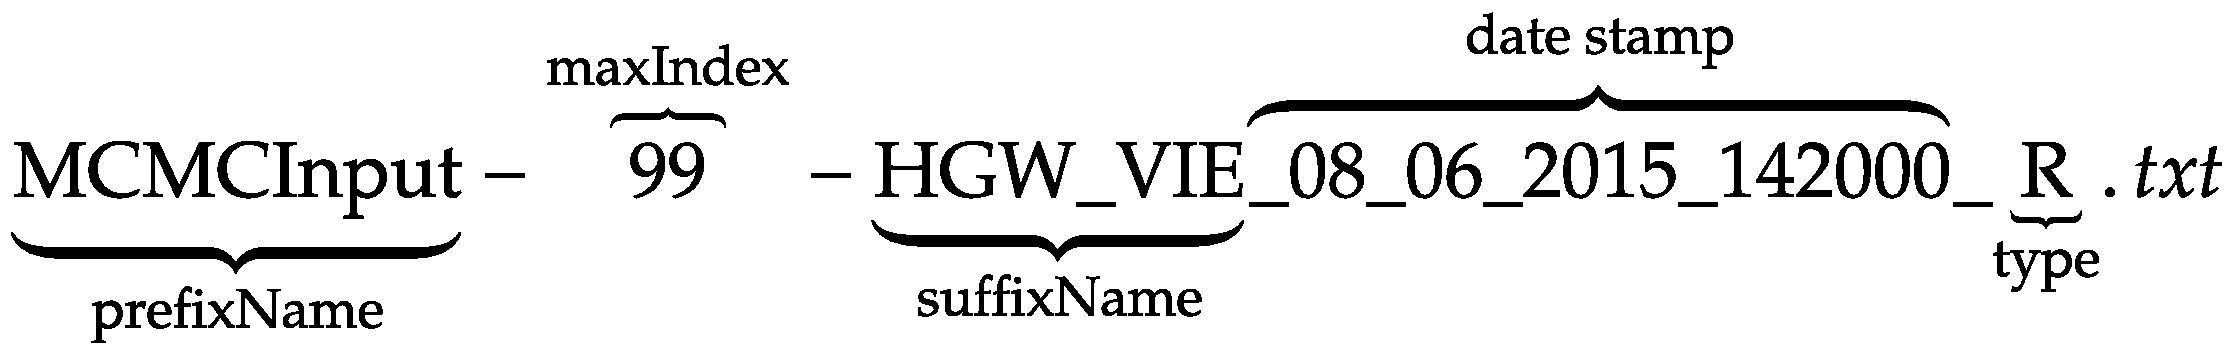
\includegraphics[width=0.65\textwidth]{MCMCOutputName.pdf}
\caption{Illustration of how to set the command line arguments for the combine scripts. \label{fig:MCMCOutputName}}
\end{figure}


\subsection{Concatenating Files}
If an MCMC analyses has been continued across multiple runs (i.e., by starting another MCMC run from the last accepted sample; see initialRC above), the 'ConcantenateData.sh' script can be used to produce a single file of all sampled growth rates 'r', initial population sizes 'c' and log-likelihoods, respectively .

{
\centering
\renewcommand{\arraystretch}{1.25}
\begin{scriptsize}
\begin{tabularx}{1\textwidth}{>{\raggedright\arraybackslash}m{1.6cm} >{\raggedright\arraybackslash}m{2.cm} >{\raggedright\arraybackslash}m{8.7cm}}
\caption{A summary of the 'combine files scripts'.}
\label{tbl:tableConcatenateScripts}\\
\toprule
\mc{1}{l}{\textbf{Script}} & \textbf{No.~of passed variables} & \textbf{Description} \\
 & & \\\hline
\mc{1}{l}{\texttt{ConcatenateDatal.sh}} & 8 &  
\hangindent=1em
\hangafter=1
\noindent


This script renames all MCMC output files, deletes the files that will not be combined, and concatenates the individual files.
To execute the script open a Shell and navigate to the folder where the scripts are stored and type

\vspace{0.05cm}
./\texttt{ConcantenateData.sh} pathToData pathToMove pathToPerlRename prefixFileName suffixFileName simIdentifier maxIndex deleteFiles .
\vspace{0.05cm}

pathToData: Provide full path to data folder.
\vspace{0.05cm}

pathToMove: Provide full path where to move data.
\vspace{0.05cm}

pathToPerlRename: Provide full path to 'rename.pl'.
\vspace{0.05cm}


prefixFileName: Provide file name prefix. For an example see Figure~\ref{fig:MCMCOutputName}.
\vspace{0.05cm}

suffixFileName: Provide file name suffix. For an example see Figure~\ref{fig:MCMCOutputName}.
\vspace{0.05cm}

simdentifier: Provide indicator for which data to concatenate: R: growth rates, C: initial population sizes, logLTS: log-likelihood
\vspace{0.05cm}

maxIndex: The number of MCMC runs the original data has been split-up to. For an example see Figure~\ref{fig:MCMCOutputName}.
\vspace{0.05cm}

deleteFiles: When set to '1' files that will not be combined will be deleted.
\vspace{0.05cm}

\end{tabularx}
\end{scriptsize}
}

Once all samples have been combined into a single file, statistics and diagnostics can be calculated by using the provided python programs \texttt{empiricIST\char`_MCMC\char`_Statistics.py} and  \texttt{empiricIST\char`_MCMC\char`_DiagSummary.py}, respectively. Taking the raw samples an input, \texttt{empiricIST\char`_MCMC\char`_Statistics.py} creates the \texttt{quantiles}- and the \texttt{Diag} files as if obtained from a single MCMC run (for detail see above). The python program \texttt{empiricIST\char`_MCMC\char`_DiagSummary.py} can then be used to create the \texttt{Diag\char`_summary} file over all individual diagnostic statistics (see above for details). Note though, that unlike the file produced from a single MCMC run, the one created by the python program does not report the standard deviation of the proposal distribution of growth rates 'r' and initial population sizes 'c', nor the acceptance ratio. Table~\ref{tbl:tablePythonStatisticsOptions} and table~\ref{tbl:tablePythonDiagOptions} give an overview of the options for each program.


{
\centering
\renewcommand{\arraystretch}{1.25}
\begin{scriptsize}
\begin{tabularx}{1\textwidth}{>{\raggedright\arraybackslash}m{1.6cm} >{\raggedright\arraybackslash}m{2.5cm} >{\raggedright\arraybackslash}m{8.2cm}}
\caption{A summary of the options of the \texttt{empiricIST\char`_MCMC\char`_Statistics.py} program.}
\label{tbl:tablePythonStatisticsOptions}\\
\toprule
\mc{1}{l}{\textbf{Short/Long option}} & \textbf{Accepted values} & \textbf{Description} \\
 & & \\\hline
\mc{1}{l}{-h, --help} & none & 
\hangindent=1em
\hangafter=1
\noindent
When the '-h'-option is invoked, a short documentation on the usage of the program is shown. Note that, if this option is invoked, the python program is not executed.
\\
\mc{1}{l}{-f, --file=} & string  &
\hangindent=1em
\hangafter=1
\noindent
The '-f'-option is a mandatory option, which passes the name of the (raw) data input file (csv formatted) to the python program. Files created by the python program will take the name of the input file and prepend \texttt{\char`_Quantiles.txt} and insert \texttt{\char`_Diag\char`_}, respectively. 
\end{tabularx}
\end{scriptsize}
}

{
\centering
\renewcommand{\arraystretch}{1.25}
\begin{scriptsize}
\begin{tabularx}{1\textwidth}{>{\raggedright\arraybackslash}m{1.6cm} >{\raggedright\arraybackslash}m{2.5cm} >{\raggedright\arraybackslash}m{8.2cm}}
\caption{A summary of the options of the \texttt{empiricIST\char`_MCMC\char`_DiagSummary.py} program.}
\label{tbl:tablePythonDiagOptions}\\
\toprule
\mc{1}{l}{\textbf{Short/Long option}} & \textbf{Accepted values} & \textbf{Description} \\
 & & \\\hline
\mc{1}{l}{-h, --help} & none & 
\hangindent=1em
\hangafter=1
\noindent
When the '-h'-option is invoked, a short documentation on the usage of the program is shown. Note that, if this option is invoked, the python program is not executed.
\\
\mc{1}{l}{-f, --file=} & string  &
\hangindent=1em
\hangafter=1
\noindent
The '-f'-option is a mandatory option, which passes the name of the (raw) data input file (csv formatted) to the python program. The output file created by the python program will take the name of the input file and prepend \texttt{\char`_summary.txt}.
\\
\mc{1}{l}{-s, --samples=} & integer  &
\hangindent=1em
\hangafter=1
\noindent
The '-s'-option is a mandatory option, which passes the number of samples to the python program. 
\end{tabularx}
\end{scriptsize}
}



\subsection{Visualization of trace data}

Additionally, there is a shell script 'FormatTracer.sh' that formats the posterior sample output file (e.g., containing the initial population size 'c' or the growth rate 'r') such that it can be read and analyzed by \textit{Tracer} \citep{RamSX14}. \textit{Tracer} is a graphical tool for visualization and diagnostics of MCMC output that, for instance, displays the posterior distribution and its credibility interval, calculates the effective sample size (ESS; note that values might be slightly different from those calculated by the \texttt{empiricIST\char`_MCMC} program since we use a more accurate but computational more intensive algorithm), and shows the trace of the posterior samples. Note that the input file is excepted to be formatted as the output file created from the \texttt{Combine\char`_PopSizes\char`_C.sh}/\texttt{Combine\char`_GrowthRates\char`_R.sh} script. Otherwise the provided \texttt{Create\char`_TailShapeFile\char`R.sh} script can be used to obtain a correctly formatted input file (please see below for details).

\vspace{0.05cm}
./\texttt{FormatTracer.sh} pathToData fileName .
\vspace{0.05cm}

pathToData: Provide full path to data folder.
\vspace{0.05cm}

fileName: Provide file name without file extension (e.g., '.txt').
\vspace{0.05cm}



\section{DFE tail shape estimation}

The growth rate posterior samples obtained from the \texttt{empiricIST\char`_MCMC} program can be used to estimate the shape of the beneficial tail of the DFE.
As part of the \emph{empiricIST} software package, we provide a python script -- \texttt{empiricIST\char`_MCMC\char`_TailShape.py} that fits a generalized pareto distribution to the observed beneficial mutations by maximizing the log-likelihood with respect to the shape and scale parameter $\kappa$ and $\psi$, respectively. Based on the shape parameter $\kappa$ one can discriminate between three different domains of attraction -- the Weibull, Gumbel and Fr\'{e}chet domain -- each corresponding to a different extreme value distribution. In biological terms, these different domains quantify the level of adaptedness of the organism in its (experimental) environment. In particular, the Gumbel domain ($\kappa=0$; null model corresponding to 'normal' level of adaptedness) is characterized by an exponential tail, whereas the Weibull domain ($\kappa<0$; better adapted) has lighter than exponential tails, and the Fr\'{e}chet domain ($\kappa>0$; less well adapted) has heavier than exponential tails. For more details please consult \cite{BeiRW07}.

While the python script primarily estimates the DFE tail shape parameter $\kappa$, there are some additional options that will be detailed here.

The general usage is as follows: After opening a command-line interface (e.g., Shell, Terminal) and navigating to the location of the \texttt{empiricIST\char`_MCMC\char`_TailShape.py} file, the program can be executed by typing

\begin{lstlisting}
python empiricIST_MCMC_TailShape.py [options] .
\end{lstlisting}

Without specifying any options the program will exit with an error and provide a short documentation on its usage, as it requires the name of the data input file (by invoking the '-f' option). 
Note that the input file needs to be formatted in a specific way. If the data set had been split into multiple subsets (see '-g' option in Tab.~\ref{tbl:tablePythonOptions}), and has been re-assembled by the using the provided shell scripts (see 'Combining Files'), the input file is already correctly formatted and there is nothing that needs to be done. However, if the data set has been analyzed as a whole (i.e., without being split into multiple subsets) the file containing the posterior growth rate samples needs to be reformatted to match the required input format.
This can be done by using he provided shell script \texttt{Create\char`_TailShapeFile\char`R.sh}, which creates the input file for the \texttt{empricIST\char`_MCMC\char`_TailShape.py} program and can be executed by opening a Shell and navigating to the folder where the scripts are stored and typing 

\vspace{0.05cm}
./\texttt{Create\char`_TailShapeFile\char`R.sh} pathToData fileName .
\vspace{0.05cm}

pathToData: Provide full path to data folder.
\vspace{0.05cm}

fileName: Provide file name without file extension (e.g., '.txt').
\vspace{0.05cm}

Note that to execute the bash script, it needs to have the appropriate rights to perform the operations. In order to set the correct permissions, open a Shell and navigate to the folder where the script is stored and type
\begin{lstlisting}[breaklines=true]
chmod 755 Create_TailShapeFile_R.sh .
\end{lstlisting}

All options and their usage of the \texttt{empricIST\char`_MCMC\char`_TailShape.py} program are given in Table~\ref{tbl:tablePythonTailShapeOptions}.

{
\centering
\renewcommand{\arraystretch}{1.25}
\begin{scriptsize}
\begin{tabularx}{1\textwidth}{>{\raggedright\arraybackslash}m{1.6cm} >{\raggedright\arraybackslash}m{2.5cm} >{\raggedright\arraybackslash}m{8.2cm}}
\caption{A summary of the options of the \texttt{empiricIST\char`_MCMC\char`_TailShape.py} program.}
\label{tbl:tablePythonTailShapeOptions}\\
\toprule
\mc{1}{l}{\textbf{Short/Long option}} & \textbf{Accepted values} & \textbf{Description} \\
 & & \\\hline
\mc{1}{l}{-h, --help} & none & 
\hangindent=1em
\hangafter=1
\noindent
When the '-h'-option is invoked, a short documentation on the usage of the program is shown. Note that, if this option is invoked, the python program is not executed.
\\
\mc{1}{l}{-f, --file=} & string  &
\hangindent=1em
\hangafter=1
\noindent
The '-f'-option is a mandatory option, which passes the name of the data input file (tsv formatted) to the python program. Files created by the python program will take the name of the input file and add option-dependent specific file identifiers. Note that even if a random data set is created (see 'r'-option), a file name must be provided since it serves as the prefix for the output file name.
\\
\mc{1}{l}{-m, --missing} & none &
\hangindent=1em
\hangafter=1
\noindent
When the '-m'-option is invoked, the distribution of measured fitnesses is shifted relative to the smallest observed selection coefficient to account for missing data (i.e., selection coefficients too small to have been observed, though this might not be a problem with EMPIRIC data).
\\
\mc{1}{l}{-s, --samples=} & integer &
\hangindent=1em
\hangafter=1
\noindent
When the '-s'-option is invoked, the python program will only consider samples with more than 'samples' beneficial mutations for maximum likelihood estimation. Note that when this option is not specified, the default is set to 10.
\\
\mc{1}{l}{-l, --lhoodrt} & none &
\hangindent=1em
\hangafter=1
\noindent 
When the '-l'-option is invoked, a likelihood-ratio test with null hypotheses $\kappa=0$ against median($\hat{\kappa}$) is performed. Note that the distribution of the test statistic is generated by using a parametric bootstrap approach with $10.000$ samples \citep[see]{BeiRW07}.
\\
\mc{1}{l}{-r, --random=} & float &
\hangindent=1em
\hangafter=1
\noindent 
When the '-r'-option is invoked, 100 random data sets are created with 100 samples each drawn from a generalized pareto distribution with scale parameter $\psi=1$ and $\kappa$ passed as command line argument.
\\
\end{tabularx}
\end{scriptsize}
}

By default the program will always create two output files that contain the $\kappa$ and $\psi$ estimates called \texttt{<InputFileName>\char`_TailShape\char`_KappaShape.txt} and\newline \texttt{<InputFileName>\char`_TailShape\char`_PsiShape.txt}, respectively. Note that even if a random data set is created (see 'r'-option), a file name must be provided since it serves as the prefix for the output file name.
When performing a likelihood-ratio test (by invoking the 'l'-option) an additional file called \texttt{<InputFileName>\char`_LRT.txt} is created containing the $\hat{\kappa}$ against which $H_0: \kappa=0$ is evaluated. Furthermore, the output file gives the maximum-likelihood estimate $\hat{\psi}_{\kappa_0}$, i.e., the estimated scale parameter $\psi$ restricting $\kappa=0$, the value of the test statistic

\begin{equation}
-2\log(\Lambda)=2(\mathcal{L}(\mathbf{X}\mid \hat{\kappa}, \hat{\psi})-\mathcal{L}(\mathbf{X}\mid o, \hat{\psi}_{\kappa_0})),
\end{equation}

where $\mathbf{X}$ denotes a single vector of posterior samples of growth rates and $\mathcal{L}$ is the log-likelihood function, and the associated p-value along with the sample size.
Note that power critically depends on sample size as has been discussed in \cite{BeiRW07} and \cite{CasS15} (the latter rather in the context of estimating $\kappa$ accurately).

\clearpage
 

\bibliography{/Users/matu/Documents/Literature/Literature.bib} 

\end{document}
